\documentclass{article}

% if you need to pass options to natbib, use, e.g.:
%     \PassOptionsToPackage{numbers, compress}{natbib}
% before loading neurips_2019

% ready for submission
% \usepackage{neurips_2019}

% to compile a preprint version, e.g., for submission to arXiv, add add the
% [preprint] option:
%     \usepackage[preprint]{neurips_2019}

% to compile a camera-ready version, add the [final] option, e.g.:
     \usepackage[final]{neurips_2019}

% to avoid loading the natbib package, add option nonatbib:
%     \usepackage[nonatbib]{neurips_2019}

\usepackage[utf8]{inputenc} % allow utf-8 input
\usepackage[T1]{fontenc}    % use 8-bit T1 fonts
\usepackage{hyperref}       % hyperlinks
\usepackage{url}            % simple URL typesetting
\usepackage{booktabs}       % professional-quality tables
\usepackage{amsfonts}       % blackboard math symbols
\usepackage{nicefrac}       % compact symbols for 1/2, etc.
\usepackage{microtype}      % microtypography

\usepackage{amsmath}        
\usepackage{booktabs}
\usepackage{multirow}
\usepackage{placeins}
\usepackage{graphicx}
\usepackage{graphbox}

\DeclareMathOperator\arctanh{arctanh}

\title{On the Vulnerability of Capsule Networks to Adversarial Attacks}
\bibliographystyle{plain}
% The \author macro works with any number of authors. There are two commands
% used to separate the names and addresses of multiple authors: \And and \AND.
%
% Using \And between authors leaves it to LaTeX to determine where to break the
% lines. Using \AND forces a line break at that point. So, if LaTeX puts 3 of 4
% authors names on the first line, and the last on the second line, try using
% \AND instead of \And before the third author name.



\author{%
  Felix Michels, Tobias Uelwer, Stefan Harmeling \\
  Department of Computer Science\\
  Heinrich-Heine University Düsseldorf\\
  \texttt{\{felix.michels, tobias.uelwer, harmeling\}@hhu.de} \\
  % examples of more authors
  \And
  Eric Upschulte \\
  Institute of Neuroscience and Medicine INM-1\\
  Forschungszentrum Jülich \\
  % Address \\
  \texttt{e.upschulte@fz-juelich.de} \\
  % \AND
  % Coauthor \\
  % Affiliation \\
  % Address \\
  % \texttt{email} \\
  % \And
  % Coauthor \\
  % Affiliation \\
  % Address \\
  % \texttt{email} \\
  % \And
  % Coauthor \\
  % Affiliation \\
  % Address \\
  % \texttt{email} \\
}
\usepackage{amsmath}
\begin{document}

\maketitle

\begin{abstract}
	In this paper we want to extensively evaluate the vulnerability of capsule networks to different adversarial attacks. Recent work suggests that these architectures are more robust towards adversarial attacks than other neural networks. However, our experiments show that capsule networks can be fooled as easily as convolutional networks.

\end{abstract}

\section{Introduction}
Capsule networks \ref{lab:capsules} have recently outperformed convolutional neural networks in terms of classification accuracy. Frost et al. \cite{darccc} also state that capsule networks are more robust against white-box adversarial attacks than other architectures. Within this work we aim to show that this is not the case. Adversarial attacks on capsule networks have been previously studied by Marchisio et al. \cite{marchisio}, however they focus on the evaluation of their method. Also Peer et al. \cite{training} have briefly discussed the application of the fast gradient sign method \cite{fgsm} on capsule networks. Detecting adversarial examples using the reconstruction quality of the capsule networks has been investigated by Frosst et al. \cite{darccc}. In this work we want to compare the results of four different attack on capsule networks trained on different datasets and examine the transferability of adversarial perturbations. This paper is structured as followed: in section \ref{lab:capsules} we recapitulate the idea of capsule networks that were introduced by Sabour et al. \cite{capsules}. In section \ref{lab:attacks} we describe the methods we used to attack the capsule networks. Section \ref{lab:experiments} summarizes the results of our experiments.

\section{Capsule Networks and Dynamic Routing}
\label{lab:capsules}
The concept of vector capsules and the dynamic routing algorithm was proposed by Sabour et al. \cite{capsules}. In an essence, neurons are grouped into vectors, so called capsules. Capsules are are meant to represent only a single specific abstract entity, for example a single object class in a classification setting.
In other words, capsules intent to develop a dedicated representation of certain characteristics in a number of dedicated vectors in favor of an entangled representation of many characteristics in a single vector, as it would be the case for MLPs or ConvNets at a given location. This allows to apply linear transformations directly to the representations of respective entities. Spatial relations, which can be implemented as a matrix product, can thus be modeled more efficiently \cite{capsules}.

The routing algorithm introduces a scalar factor, the so called routing coefficient, for each connection between a capsule $i$ from a layer $L$ and capsule $j$ from layer $L+1$. These coefficients explicitly regulate the influence that previous capsules may have on a given capsule $j$ and are determined by the dynamic routing procedure. As this procedure implements a \textit{routing by agreement} mechanism, it yields high coefficients if a capsule $j$ matches the expectation of a capsule $i$ and low coefficients otherwise. [TODO: clarify] Theoretically, that means information flows where it is needed, both during forward and backpropagation. This also supports the goal of capsules with a dedicated representation.

[TODO: Layer (primary, dense?, convcaps)]

[NOTE: text in A.E.]



\section{Adversarial Attacks}
\label{lab:attacks}

Adversarial attacks can be performed in different settings: in the white-box setting the attacker can compute the gradient of the networks output with respect to the input, whereas in the black-box setting such calculations are not possible. Furthermore, adversarial attacks can be classified into targeted attacks, where the goal of the attack is that the network assigns a given label to the manipulated image, and untargeted attacks, where the attacker's goal is to fool the network in the sense that it only missclassifies a given image.

Throughout this paper we denote the input image as $x\in [0,1]^{n\times n}$, the neural network's output logits as $Z$ and the perturbation as $\delta$. \\
% Explain this better
If $F$ is the output of the network interpretable as probability, then\\
$F(x) = softmax (Z(x))$ in the case of the CNN\\
$Z(x) = \arctanh(2 \cdot F(x) - 1)$ in the case of the CapsNet\\
$C(x)$ refers to the label assigned to $x$ by the network and $C^*(x)$ is the correct label of $x$. Furthermore, we refer to the i-the entry of $Z(x)$ as $Z(x)_i$.

\subsection{Carlini-Wagner Attack}

The Carlini-Wagner attack \cite{carlini} is a targeted white-box attack and performed by solving the following constrained optimization problem
\begin{equation}
	\begin{aligned}
	& \underset{\delta}{\text{minimize}}
	& & ||\delta||_2 + c \cdot \max(\max_{i\neq t}(Z(x+\delta)_i)-Z(x)_t, -\kappa) \\
	& \text{subject to}
	& & x+\delta \in [0,1]^{n \times n},
	\end{aligned}
\end{equation}

where $\kappa > 0$ controlls the confidence $c>0$. The optimal value for c (i.e. the smallest value, that results in an adversarial example) is found using a binary search. To ensure the box-constraint on $x+\delta$ the authors suggested the following transform of variables 
\begin{equation}
	\delta = \frac{1}{2}(\tanh(w)+1)-x,
\end{equation} 
where the $\tanh$-function is applied componentwise. After this transformation the optimization problem is treated as unconstrained and can be solved in terms of $w$ using Adam \cite{adam}. In their work Carlini and Wagner also proposed two different approaches to handle the box-constraint: projected gradient descent and clipped gradient descent. For details we refer the reader to the original work \cite{carlini}.

\subsection{Boundary Attack}

The idea of the boundary attack as it was introduced by Brendel et al. \cite{boundary} is to sample a perturbation which leads to a missclassification of the original image $x^{(0)}:=x$. Additionally, the desired perturbation should have the smallest possible norm. The initial perturbation $\delta^{(0)}$ is componentwise sampled from a uniform distribution $\delta^{(0)}_{ij}\sim \mathcal{U}(0,1)$. Initial perturbations, which are not missclassified, are rejected. During the attack adversarial images are constructed iteratively $x^{(k+1)}:= x^{(k)}+\delta^{(k)}$ by a random walk close to the decision boundary. During this random walk the following three conditions are enforced by appropriate scaling and clipping of the image and the perturbation:
\begin{enumerate}
	\item The new image $x^{(k+1)}$ should be in the range of a valid image, i.e. in $x^{(k+1)}\in [0,1]^{n\times n}$.
	\item The proportion of the size of the perturbation $\delta^{(k)}$ and the distance to the given image equal to a given parameter $\gamma$.
	\item The reduction of the distance from the adversarial image to the original image $d(x, x^{(k)})-d(x, x^{(k+1)})$ is proportional to $d(x, x^{(k)})$ with $\nu>0$.
\end{enumerate}
The parameters $\gamma$ and $\nu$ are adjusted dynamically, similarly to Trust Region methods.


\subsection{DeepFool Attack}
Deepfool is an untargeted white-box attack developed by Moosavi-Dezfooli eta al \cite{deepfool}.
The authors found, that minimal adversarial perturbations for affine multiclass classifier can be computed exactly and quickly,
by calculated the distance to the (linear) decision boundaries and making an orthogonal projection to the nearest one.
Deepfool initializes $\delta \gets 0$ and then iteratively approximates $F$ with its first degree Taylor polynomial at $x + \delta$, computes a perturbation $\Delta \delta$ for this approximation as described above and updates $\delta \gets \delta + \Delta \delta$.
For better results, we restrict the norm of $\Delta \delta$ each step.

\subsection{Universal Adversarial Perturbations}
A universal perturbation is a single vector $\delta \in \mathbb{R}^{n\times n}$, such that $C(x + \delta) \neq C^*(x)$ for multiple $x$ sampled from the input image distribution. This concept was proposed by Moosave-Dezfooli et al. \cite{universal} and we use a variation of their algorithm:
\begin{enumerate}
	\item Initialize $\delta \gets 0$.
	\item Choose a batch $X = \{x_1, ..., x_N\}$ of images with $\forall x_i \in\ X:  C(x_i + \delta) = C^*(x_i)$.
	\item For each $x_i$ compute a perturbation $\delta_i$ using FGSM \cite{fgsm}.
	\item Update the perturbation: $\delta \gets \delta + \frac{1}{N} \sum\limits_{i=0}^N \delta_i$
	\item Clip $\delta$ to a maximal norm chosen beforehand.
\end{enumerate}
Since this method depends on the FGSM \cite{fgsm} it is a white-box attack.


\section{Experiments}
\label{lab:experiments}

\subsection{Datasets and Network Architectures}

We train the capsule network on the following benchmark datasets: MNIST \cite{mnist}, Fashion-MNIST \cite{fashion}, SVHN \cite{svhn} and CIFAR-10 \cite{cifar}. Each dataset is divided into ten different classes. 
As a baseline architecture we use a convolutional neural network (CNN) which we trained on each of the datasets while using batch-normalization \cite{batchnorm} and dropout \cite{dropout}. Since training capsule networks (CapsNets) is in practice rather difficult, we adapt different architectures for each datasets: For the CIFAR-10 dataset we use an architecture with ... primary capsules and .... For the other datasets we used a smaller architecture.
Mnist: 3 layer network, like sabour \cite{capsules} did, but only 64 convolutional kernels in the first layer
Fashion-Mnist: Two convolutional layers at the beginning
SVHN: Two convolutional layers at the beginning, also bigger capsules and bigger reconstruction network
Cifar10: CapsNets have problems with more complex data \cite{complex}, we use a modified DCNet \cite{denseanddiverse} with three capsule layers and "none-of-the-above" category for the dynamic routing \cite{capsules}

For each dataset:\\
DeepFool and Boundary attack: 1000 adversarial examples on images randomly chosen from the test set\\
Carlini-Wagner: 500 adversarial examples, with $\kappa = 1$, on images randomly chosen from the test set. Target labels not equal to true label, otherwise random \\
Universal Perturbation: Split the test set in 10 parts, compute 10 adversarial perturbations on each part, stop once accuracy is below 50\%. However, each perturbation is evaluated on the whole test set.

%\begin{itemize}
%	\item MNIST: $28\times28$ grayscale images of digits (60,000  images for training/10,000  images for testing) \cite{mnist}
%	\item Fashion-MNIST:  $28\times28$ grayscale images of fashion items (60,000 images for training/images 10,000 for testing) \cite{fashion}
%	\item SVHN: $32\times32$ color images of house numbers (73,257  images for training/26,032  images for testing) \cite{svhn}
%	\item CIFAR10: $32\times32$ color images (50.000  images for training/10.000  images for testing) \cite{cifar}
%\end{itemize}

\subsection{Results}

We are aware of the fact that the test accuracies of our models are not state-of-the-art. However, we found our models to be suitable for the given task, since the similar performances of convolutional and capsule networks ensure comparability.

\begin{table}[h]
	\caption{Test accuracies achieved by our networks.}
	\centering
	\begin{tabular}{lcccc}
		\toprule
		Network       & MNIST & Fashion-MNIST & SVHN & CIFAR10  \\
		\midrule
		Convolutional neural network & 99.4\% & 92.8\% & 92.6\% & 82.6\% \\
		Capsule network            & 99.4\% & 92.6\% & 92.4\% & 82.4\% \\
		\bottomrule\\
	\end{tabular}
	\label{tab:accuracies}
\end{table}

\begin{table}[h]
	\caption{Test accuracies on adversarial examples.}
	\centering
	\begin{tabular}{llcccc}
		\toprule
		Attack & Network       & MNIST & Fashion-MNIST & SVHN & CIFAR10  \\
		\midrule
		\multirow{2}{*}{CW} & CNN &  &  &  &  \\
		& CapsNet            &  &  &  &  \\
		\midrule
		\multirow{2}{*}{Boundary} & CNN &  &  &  &  \\
		& CapsNet            &  &  &  &  \\
		\midrule
		\multirow{2}{*}{DeepFool} & CNN &  &  &  &  \\
		& CapsNet           &  &  &  &  \\
		\midrule
		\multirow{2}{*}{Universal} & CNN &  &  &  &  \\
		& CapsNet           &  &  &  &  \\
		\bottomrule\\
	\end{tabular}
	\label{tab:attacks}
\end{table}

\begin{table}[h]
	\caption{Comparison of the average perturbation norm for each attack and architecture.}
	\centering
	\begin{tabular}{llcccc}
		\toprule
		Attack & Network       & MNIST & Fashion-MNIST & SVHN & CIFAR10  \\
		\midrule
		\multirow{2}{*}{CW} & CNN & 1.4 & 0.51 & 0.67 & 0.56 \\
		& CapsNet            & 1.8 & 0.5 & 0.60 & 0.37 \\
		\midrule
		\multirow{2}{*}{Boundary} & CNN & 3.07 & 1.24 & 2.42 & 1.76 \\
		& CapsNet            & 3.26 & 0.93 & 1.88 & 0.99 \\
		\midrule
		\multirow{2}{*}{DeepFool} & CNN & 1.08 & 0.32 & 0.43 & 0.26 \\
		& CapsNet           & 1.99 & 0.57 & 0.78 & 0.19 \\
		\midrule
		\multirow{2}{*}{Universal} & CNN & 0.921 & 1.22 & 2.61 & 3.0 \\
		& CapsNet           & 0.921 & 1.22 & 2.61 & 3.0 \\
		\bottomrule\\
	\end{tabular}
	\label{tab:norms}
\end{table}

\begin{table}[h]
	\centering
	\begin{tabular}{rlll} 
	CW & 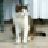
\includegraphics[height=1.5cm, align=c]{figures/carlini_wagner_orig.pdf} & 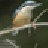
\includegraphics[height=1.5cm, align=c]{figures/carlini_wagner_adversarial.pdf} & 
\includegraphics[height=1.5cm, align=c]{figures/carlini_wagner_diff.pdf}\\
	\\
	Boundary & 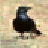
\includegraphics[height=1.5cm, align=c]{figures/boundary_orig.pdf} & 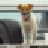
\includegraphics[height=1.5cm, align=c]{figures/boundary_adversarial.pdf} & 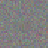
\includegraphics[height=1.5cm, align=c]{figures/boundary_diff.pdf}\\
	\\
	DeepFool & 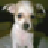
\includegraphics[height=1.5cm, align=c]{figures/deepfool_orig.pdf} & 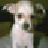
\includegraphics[height=1.5cm, align=c]{figures/deepfool_adversarial.pdf} & 
\includegraphics[height=1.5cm, align=c]{figures/deepfool_diff.pdf}\\
	\\
	Universal & 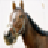
\includegraphics[height=1.5cm, align=c]{figures/universal_orig.pdf} & 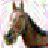
\includegraphics[height=1.5cm, align=c]{figures/universal_adversarial.pdf} & 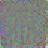
\includegraphics[height=1.5cm, align=c]{figures/universal_diff.pdf}\\
	\\
	\vspace{0.1cm}\\
	\end{tabular}
	\label{tab:images}
	\caption{Original images from the CIFAR10 dataset (left), adversarial images (middle) and the corresponding perturbation (right) calculated for a capsule network.}
\end{table}

\subsection{Visualizing Universal Perturbations}

We also visualized the universal perturbations calculated for the CapsNet and for the CNN using t-SNE \cite{tsne} and we observe that the perturbations for the CapsNet seem to be inherently different than the perturbations for the convolutional networks.
\begin{figure}
	\centering
	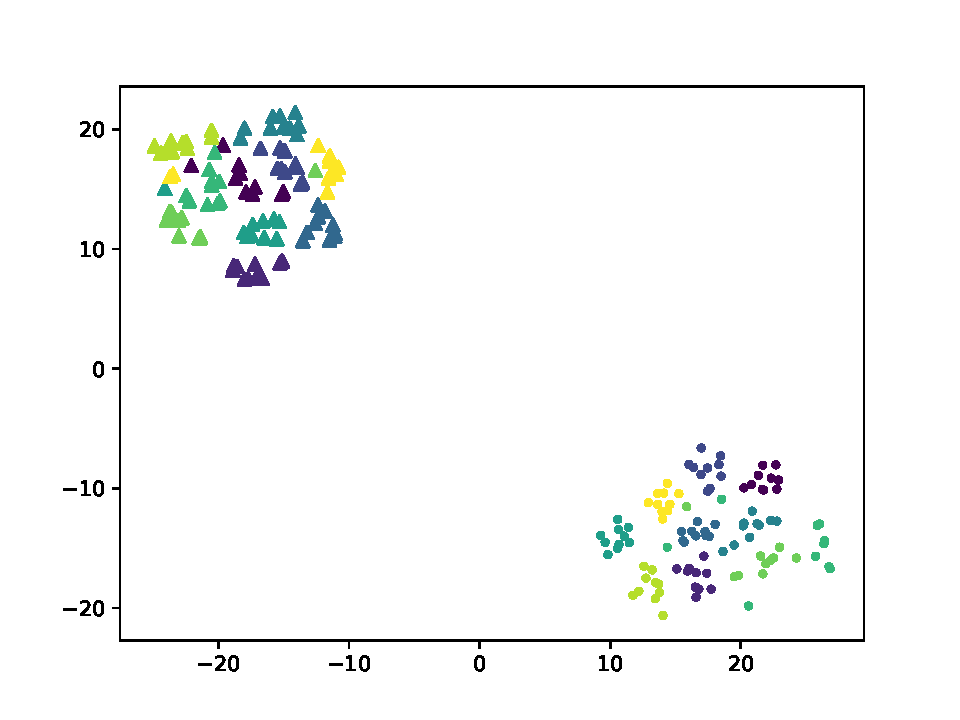
\includegraphics[height=5.5cm]{figures/tsne.pdf}
	\caption{Two dimensional embedding of the universal perturbations calculated using t-SNE \cite{tsne}. The upper right cluster represents perturbations calculated on a CNN, whereas the lower left cluster represents those calculated on a CapsNet. Perturbations with the same color were created using the same subset of test data.}
\end{figure}


\FloatBarrier
\section{Conclusion}
Our experiments show that capsule networks are as vulnerable to (white-box) attacks as convolutional architectures.


\bibliography{neurips_2019}


\end{document}
